\chapter{TCP输入}
\label{chapter:tcp_input}
	\section{Linux内核网络数据接收流程概览}
        \begin{figure}[htb]        
            \centering
            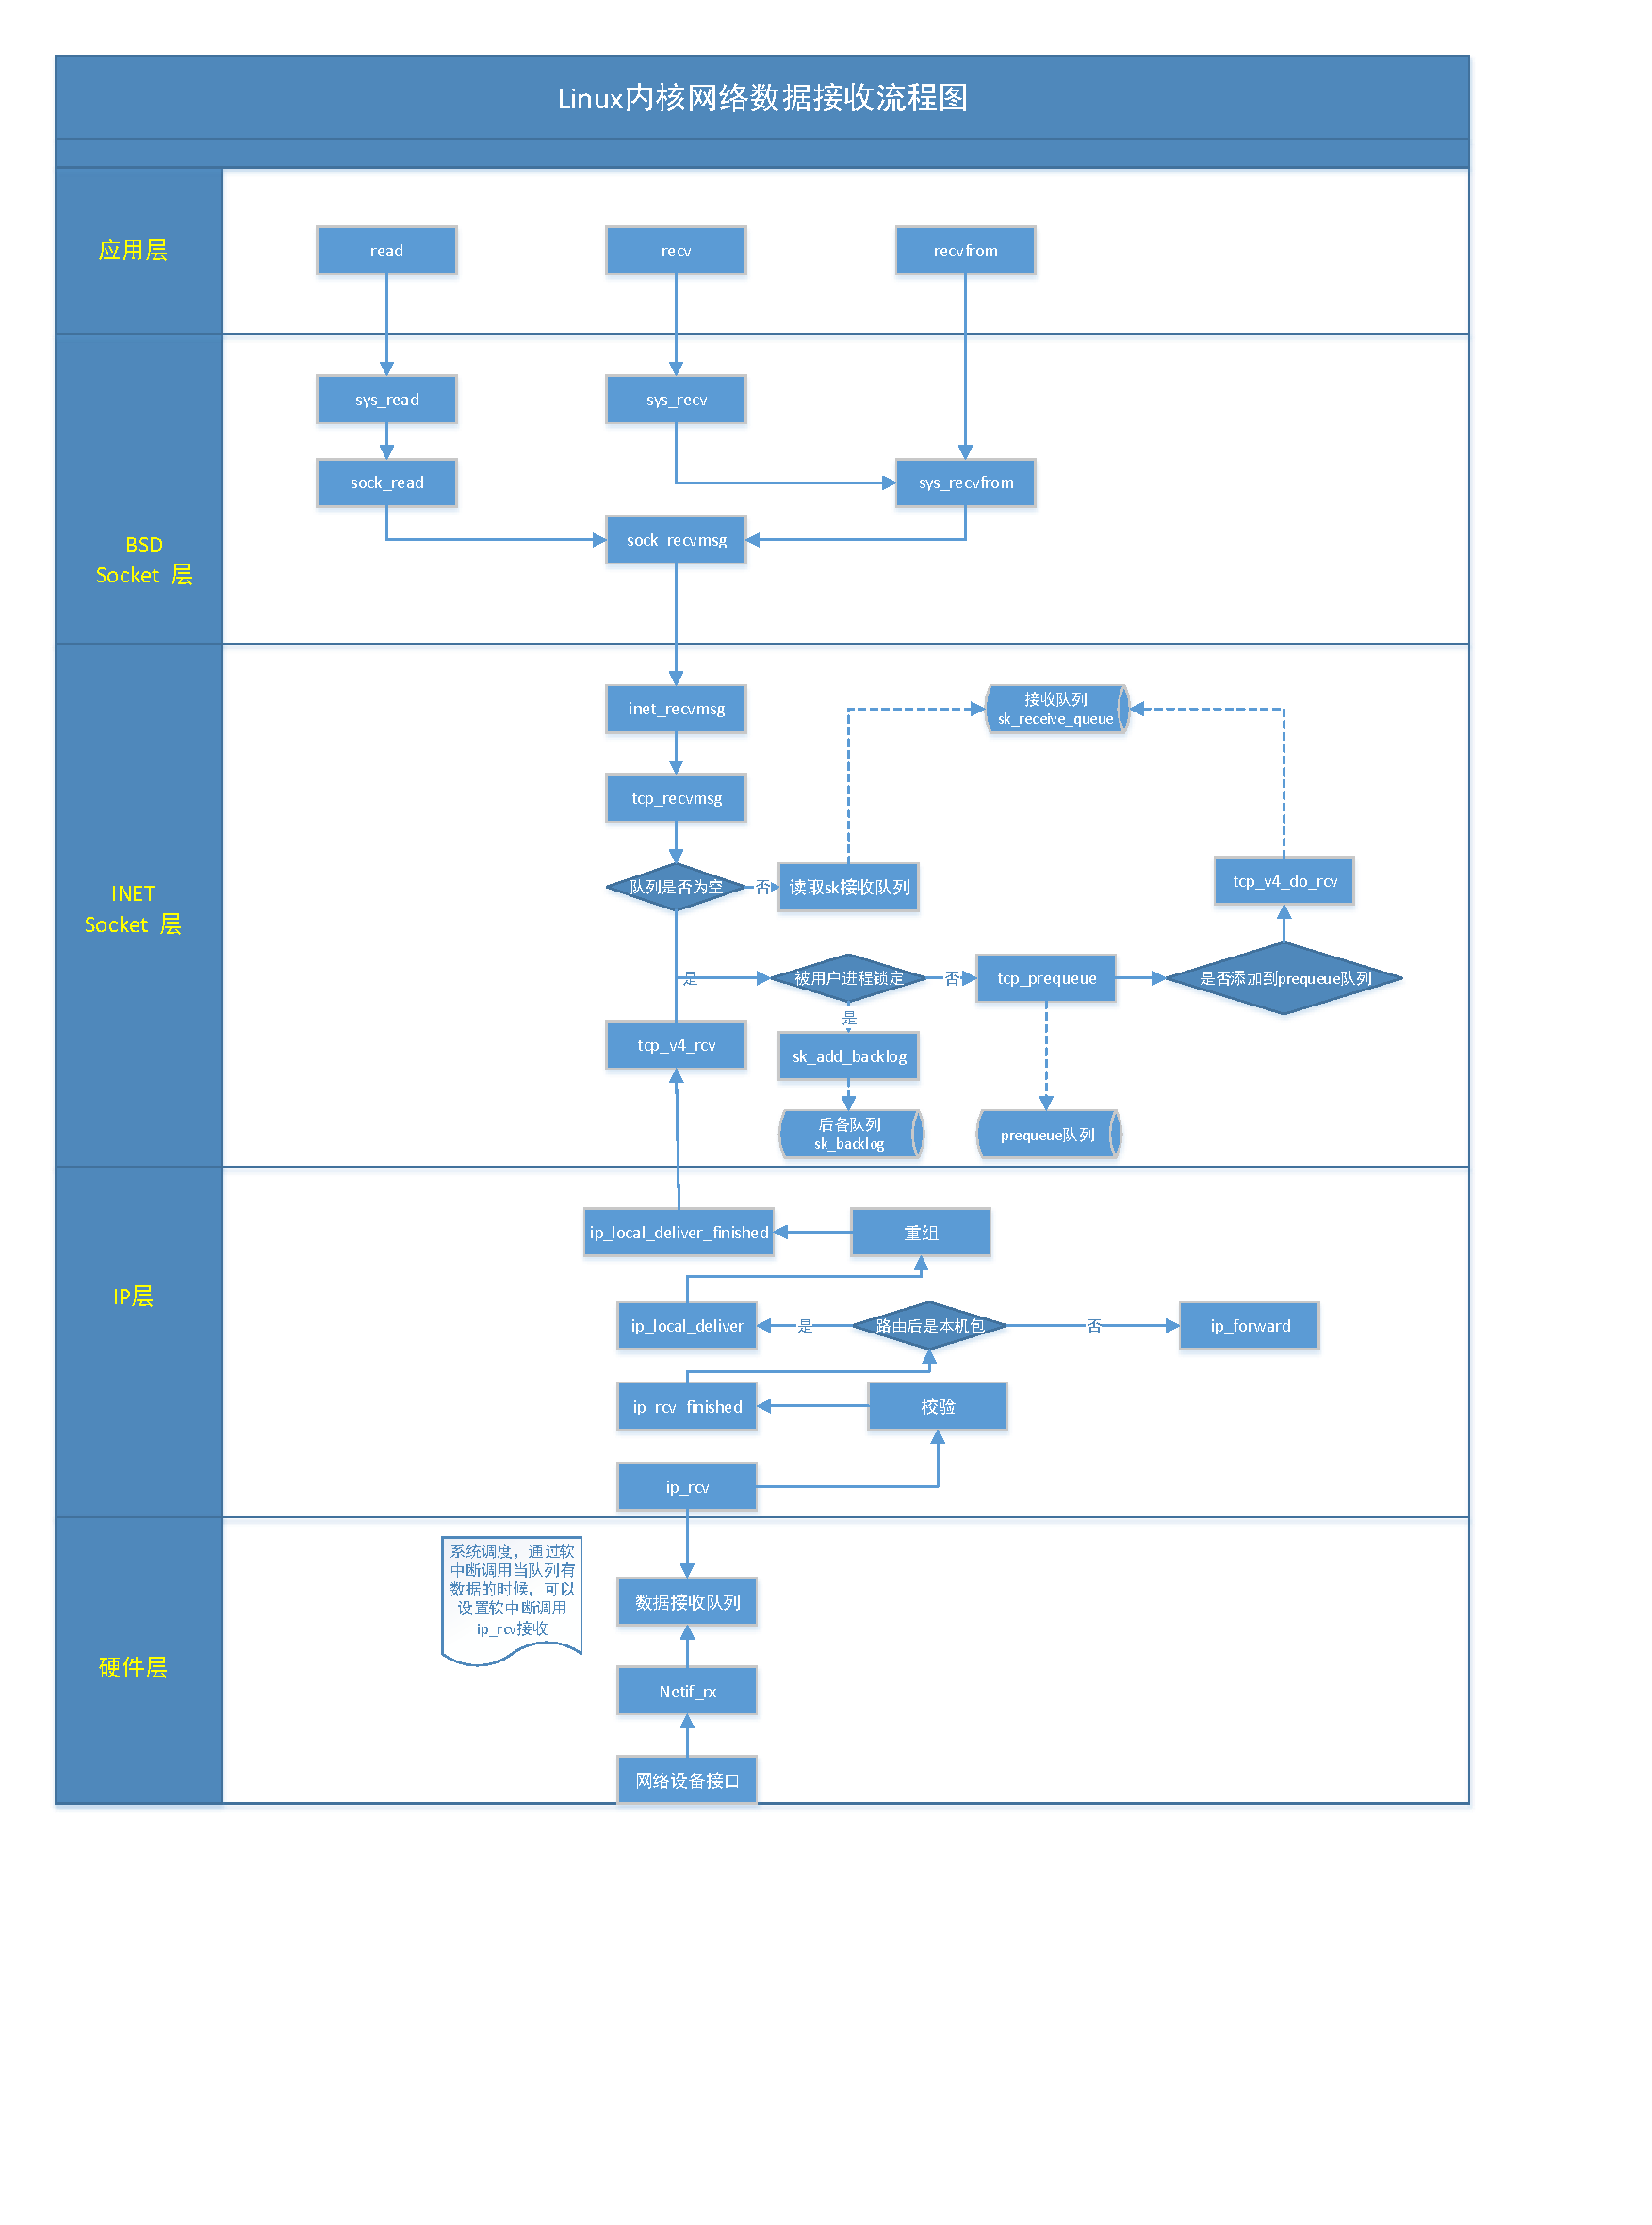
\includegraphics[width=\textwidth]  {images/Linux Network Receive.pdf}
        \end{figure}    
		正如上图所示,Linux内核的网络数据接收时分为以上5个层次的。
		每个层次都有自己功能,相互依赖,同时又独立成块。
		下面,我们来依次介绍这些层次。
\begin{enumerate}
\item[应用层]			对于应用层来说,提供多种接口来接收数据,包括read,recv,recvfrom.
\item[BSD Socket层]		这一层主要是在应用层进行进一步的处理。
\item[INET Socket层]		当被IP层的函数调用的时候,如果发现用户进程因正在操作传输控制块而将其锁定
						就会将未处理的TCP段添加到后备队列中,而一旦用户进程解锁传输控制块,就会理解处理
						后备队列,将TCP段处理之后的直接添加到接收队列中。
						当被BSD Socket的函数调用的时候,此时说明用户此时需要数据,那么我们就利用tcp\_recvmsg来
						进行消息接收,当然,起初得判断队列是否为空,不为空才可以直接处理,为空就得进一步进行相关的处理。
\item[IP层]
				IP层则主要是在系统调度的时候,根据数据接收队列中是否由数据进行进一步的检验,
				判断该包是不是发往该主机。然后进行数据包的重组(这是因为TCP数据有可能因为太大而被分片),
				然后调用INET层的函数进行进一步的处理。
\item[硬件层]     这一部分主要是网卡接收到数据之后,进行发出请求中断,
				  然后调用相关函数进行处理,将接收到的数据放入到数据接收队列中。
					当然,这时,那些没有经过FCS检验过的数据包这时候已经被抛弃了。
\end{enumerate}

		而在本文的分析中,我们主要关注的时TCP层的实现,故而我们主要分析INET Socket层。
	\section{自底向上调用与自顶向下调用}
		\subsection{自底向上处理}
			\subsubsection{\mintinline{C}{tcp_v4_rcv}}
\begin{minted}[linenos]{C}
int tcp_v4_rcv(struct sk_buff *skb)
{
	const struct iphdr *iph;
	const struct tcphdr *th;
	struct sock *sk;
	int ret;
	struct net *net = dev_net(skb->dev);

	if (skb->pkt_type != PACKET_HOST)
		goto discard_it;

	/* Count it even if it's bad */
	TCP_INC_STATS_BH(net, TCP_MIB_INSEGS);

	if (!pskb_may_pull(skb, sizeof(struct tcphdr)))
		goto discard_it;

	th = tcp_hdr(skb);

	if (th->doff < sizeof(struct tcphdr) / 4)
		goto bad_packet;
	if (!pskb_may_pull(skb, th->doff * 4))
		goto discard_it;

	/* An explanation is required here, I think.
	 * Packet length and doff are validated by header prediction,
	 * provided case of th->doff==0 is eliminated.
	 * So, we defer the checks. */

	if (skb_checksum_init(skb, IPPROTO_TCP, inet_compute_pseudo))
		goto csum_error;

	th = tcp_hdr(skb);
	iph = ip_hdr(skb);
	/* This is tricky : We move IPCB at its correct location into TCP_SKB_CB()
	 * barrier() makes sure compiler wont play fool^Waliasing games.
	 */
	memmove(&TCP_SKB_CB(skb)->header.h4, IPCB(skb),
		sizeof(struct inet_skb_parm));
	barrier();

	TCP_SKB_CB(skb)->seq = ntohl(th->seq);
	TCP_SKB_CB(skb)->end_seq = (TCP_SKB_CB(skb)->seq + th->syn + th->fin +
				    skb->len - th->doff * 4);
	TCP_SKB_CB(skb)->ack_seq = ntohl(th->ack_seq);
	TCP_SKB_CB(skb)->tcp_flags = tcp_flag_byte(th);
	TCP_SKB_CB(skb)->tcp_tw_isn = 0;
	TCP_SKB_CB(skb)->ip_dsfield = ipv4_get_dsfield(iph);
	TCP_SKB_CB(skb)->sacked	 = 0;

lookup:
	sk = __inet_lookup_skb(&tcp_hashinfo, skb, th->source, th->dest);
	if (!sk)
		goto no_tcp_socket;

process:
	if (sk->sk_state == TCP_TIME_WAIT)
		goto do_time_wait;

	if (sk->sk_state == TCP_NEW_SYN_RECV) {
		struct request_sock *req = inet_reqsk(sk);
		struct sock *nsk;

		sk = req->rsk_listener;
		if (unlikely(tcp_v4_inbound_md5_hash(sk, skb))) {
			reqsk_put(req);
			goto discard_it;
		}
		if (unlikely(sk->sk_state != TCP_LISTEN)) {
			inet_csk_reqsk_queue_drop_and_put(sk, req);
			goto lookup;
		}
		sock_hold(sk);
		nsk = tcp_check_req(sk, skb, req, false);
		if (!nsk) {
			reqsk_put(req);
			goto discard_and_relse;
		}
		if (nsk == sk) {
			reqsk_put(req);
		} else if (tcp_child_process(sk, nsk, skb)) {
			tcp_v4_send_reset(nsk, skb);
			goto discard_and_relse;
		} else {
			sock_put(sk);
			return 0;
		}
	}
	if (unlikely(iph->ttl < inet_sk(sk)->min_ttl)) {
		NET_INC_STATS_BH(net, LINUX_MIB_TCPMINTTLDROP);
		goto discard_and_relse;
	}

	if (!xfrm4_policy_check(sk, XFRM_POLICY_IN, skb))
		goto discard_and_relse;

	if (tcp_v4_inbound_md5_hash(sk, skb))
		goto discard_and_relse;

	nf_reset(skb);

	if (sk_filter(sk, skb))
		goto discard_and_relse;

	skb->dev = NULL;

	if (sk->sk_state == TCP_LISTEN) {
		ret = tcp_v4_do_rcv(sk, skb);
		goto put_and_return;
	}

	sk_incoming_cpu_update(sk);

	bh_lock_sock_nested(sk);
	tcp_sk(sk)->segs_in += max_t(u16, 1, skb_shinfo(skb)->gso_segs);
	ret = 0;
	if (!sock_owned_by_user(sk)) {
		if (!tcp_prequeue(sk, skb))
			ret = tcp_v4_do_rcv(sk, skb);
	} else if (unlikely(sk_add_backlog(sk, skb,
					   sk->sk_rcvbuf + sk->sk_sndbuf))) {
		bh_unlock_sock(sk);
		NET_INC_STATS_BH(net, LINUX_MIB_TCPBACKLOGDROP);
		goto discard_and_relse;
	}
	bh_unlock_sock(sk);

put_and_return:
	sock_put(sk);

	return ret;

no_tcp_socket:
	if (!xfrm4_policy_check(NULL, XFRM_POLICY_IN, skb))
		goto discard_it;

	if (tcp_checksum_complete(skb)) {
csum_error:
		TCP_INC_STATS_BH(net, TCP_MIB_CSUMERRORS);
bad_packet:
		TCP_INC_STATS_BH(net, TCP_MIB_INERRS);
	} else {
		tcp_v4_send_reset(NULL, skb);
	}

discard_it:
	/* Discard frame. */
	kfree_skb(skb);
	return 0;

discard_and_relse:
	sock_put(sk);
	goto discard_it;

do_time_wait:
	if (!xfrm4_policy_check(NULL, XFRM_POLICY_IN, skb)) {
		inet_twsk_put(inet_twsk(sk));
		goto discard_it;
	}

	if (tcp_checksum_complete(skb)) {
		inet_twsk_put(inet_twsk(sk));
		goto csum_error;
	}
	switch (tcp_timewait_state_process(inet_twsk(sk), skb, th)) {
	case TCP_TW_SYN: {
		struct sock *sk2 = inet_lookup_listener(dev_net(skb->dev),
							&tcp_hashinfo,
							iph->saddr, th->source,
							iph->daddr, th->dest,
							inet_iif(skb));
		if (sk2) {
			inet_twsk_deschedule_put(inet_twsk(sk));
			sk = sk2;
			goto process;
		}
		/* Fall through to ACK */
	}
	case TCP_TW_ACK:
		tcp_v4_timewait_ack(sk, skb);
		break;
	case TCP_TW_RST:
		goto no_tcp_socket;
	case TCP_TW_SUCCESS:;
	}
	goto discard_it;
}
\end{minted}
		\subsection{自顶向下处理}
			\subsubsection{\mintinline{C}{tcp_recvmsg}}
				我们一步一步对该函数进行分析。
\begin{minted}[linenos]{C}
/*
Location:

	net/ipv4/tcp.c

Function:

 *	This routine copies from a sock struct into the user buffer.
 *
 *	Technical note: in 2.3 we work on _locked_ socket, so that
 *	tricks with *seq access order and skb->users are not required.
 *	Probably, code can be easily improved even more.

Parameter:

	sk:传输控制块。
	msg:
	len:
	nonblock:
	flags:读取数据的标志。
	addrlen:
*/

int tcp_recvmsg(struct sock *sk, struct msghdr *msg, size_t len, int nonblock,
		int flags, int *addr_len)
{
	struct tcp_sock *tp = tcp_sk(sk);
	int copied = 0;
	u32 peek_seq;
	u32 *seq;
	unsigned long used;
	int err;
	int target;		/* Read at least this many bytes */
	long timeo;
	struct task_struct *user_recv = NULL;
	struct sk_buff *skb, *last;
	u32 urg_hole = 0;
	//如果只是为了接收来自套接字错误队列的错误,那就直接执行如下函数。
	if (unlikely(flags & MSG_ERRQUEUE))
		return inet_recv_error(sk, msg, len, addr_len);
	//不是特别理解,,????
	if (sk_can_busy_loop(sk) && skb_queue_empty(&sk->sk_receive_queue) &&
	    (sk->sk_state == TCP_ESTABLISHED))
		sk_busy_loop(sk, nonblock);
\end{minted}
上述主要处理一些比较异常的情况,接下来就开始进行正常的处理了。
\begin{minted}[linenos]{C}
	/*
		在用户进程进行读取数据之前,必须对传输层进行加锁,这主要时为了在读的过程中,软中断
		操作传输层,从而造成数据的不同步甚至更为严重的不可预料的结果。
	*/
	lock_sock(sk);
	//初始化错误码,Transport endpoint is not connected
	err = -ENOTCONN;
	/*
		如果此时只是处于LISTEN状态,表明尚未建立连接,
		此时不允许用户读取数据,只能返回。
	*/
	if (sk->sk_state == TCP_LISTEN)
		goto out;
	/*
		获取阻塞读取的超时时间,如果进行非阻塞读取,则超时时间为0。
	*/
	timeo = sock_rcvtimeo(sk, nonblock);

	/* Urgent data needs to be handled specially. 
		如果是要读取带外数据,则需要跳转到recv_urg进行处理。
	*/
	if (flags & MSG_OOB)
		goto recv_urg;
\end{minted}
	继续处理。
\begin{minted}[linenos]{C}
	//被修复了???啥意思》?》
	if (unlikely(tp->repair)) {
		//	Operation not permitted
		err = -EPERM;
		//如果只是查看数据的话,就直接跳转到out处理
		if (!(flags & MSG_PEEK))
			goto out;
		//????
		if (tp->repair_queue == TCP_SEND_QUEUE)
			goto recv_sndq;
		//Invalid argument
		err = -EINVAL
		if (tp->repair_queue == TCP_NO_QUEUE)
			goto out;

		/* 'common' recv queue MSG_PEEK-ing */
	}
\end{minted}
	
	接下来进行数据复制。在把数据从接收缓存复制到用户空间的过程中,
	会更新当前已复制为止,以及段序号。如果接收数据,则会更新copied\_seq,
	但是如果只是查看数据而并不是从系统缓冲区移走数据,那么不能更新copied\_seq。
	因此,数据复制到用户空间的过程中,区别接收数据还是查看数据是根据是否更新copied\_seq,
	所以这里时根据接收数据还是查看来获取要更新标记的地址,而后面的复制操作就完全不关心时接收
	还是查看。
	
	最后一行调用相关函数根据是否设置了MSG\_WAITALL来确定本次调用需要接收数据的长度。如果设置
	了MSG\_WAITALL标志,则读取数据长度为用户调用时输入的参数len。
\begin{minted}[linenos]{C}
	seq = &tp->copied_seq;
	if (flags & MSG_PEEK) {
		peek_seq = tp->copied_seq;
		seq = &peek_seq;
	}

	target = sock_rcvlowat(sk, flags & MSG_WAITALL, len);
\end{minted}

	接下来通过urg\_data和urg\_seq来检测当前是否读取到带外数据。如果在
	读带外数据,则终止本次正常数据的读取。否则,如果用户进程有信号待处理,
	则也终止本次的读取。
\begin{minted}[linenos]{C}
	do {
		u32 offset;

		/* Are we at urgent data? Stop if we have read anything or have SIGURG pending. */
		if (tp->urg_data && tp->urg_seq == *seq) {
			if (copied)
				break;
			if (signal_pending(current)) {
				copied = timeo ? sock_intr_errno(timeo) : -EAGAIN;
				break;
			}
		}
\end{minted}

	接下来首先获取一个缓存区。
\begin{minted}[linenos]{C}
		/* Next get a buffer. */
		//接下来获取下一个要读取的的段。
		last = skb_peek_tail(&sk->sk_receive_queue);
		skb_queue_walk(&sk->sk_receive_queue, skb) {
			last = skb;
			/* Now that we have two receive queues this
			 * shouldn't happen.
				如果接收队列中的段序号比较大,则说明也获取不到下一个待获取的段,
				这样也只能接着处理prequeue或后备队列,实际上这种情况不应该发生。
			 */
			if (WARN(before(*seq, TCP_SKB_CB(skb)->seq),
				 "recvmsg bug: copied %X seq %X rcvnxt %X fl %X\n",
				 *seq, TCP_SKB_CB(skb)->seq, tp->rcv_nxt,
				 flags))
				break;
			/*
				到此,我们已经获取了下一个要读取的数据段,计算该段开始读取数据的偏移位置,
				当然,该偏移值必须在该段的数据长度范围内才有效。
			*/
			offset = *seq - TCP_SKB_CB(skb)->seq;	
			/*
				由于SYN标志占用了一个序号,因此如果存在SYN标志,则需要调整
				偏移。由于偏移offset为无符号整型,因此,不会出现负数的情况。
			*/
			if (TCP_SKB_CB(skb)->tcp_flags & TCPHDR_SYN)
				offset--;
			/*
				只有当偏移在该段的数据长度范围内,才说明待读的段才是有效的,因此,接下来
				跳转到found_ok_skb标签处读取数据。
			*/
			if (offset < skb->len)
				goto found_ok_skb;
			/*
				如果接收到的段中有FIN标识,则跳转到found_fin_ok处处理。
			*/
			if (TCP_SKB_CB(skb)->tcp_flags & TCPHDR_FIN)
				goto found_fin_ok;
			WARN(!(flags & MSG_PEEK),
			     "recvmsg bug 2: copied %X seq %X rcvnxt %X fl %X\n",
			     *seq, TCP_SKB_CB(skb)->seq, tp->rcv_nxt, flags);
		}
\end{minted}

	只有在读取完数据后,才能在后备队列不为空的情况下区处理接收到后备队列中的TCP段。
	否则终止本次读取。

	由于是因为用户进程对传输控制块进行的锁定,将TCP段缓存到后备队列,故而,一旦用户进程释放传输控制块就应该立即处理后备队列。
	处理后备队列直接在release\_sock中实现,以确保在任何时候解锁传输控制块时能立即处理后备队列。
\begin{minted}[linenos]{C}
		/* Well, if we have backlog, try to process it now yet. */

		if (copied >= target && !sk->sk_backlog.tail)
			break;
\end{minted}

	当接收队列中可以读取的段已经读完,在处理prequeue或后备队列之前,我们需要显检查是否会存在一些
	异常的情况,如果存在这类情况,就需要结束这次读取,返回前当然还顺便检测后备队列是否存在数据,如果有
	则还需要处理。	
\begin{minted}[linenos]{C}
		if (copied) {
			/*
				检测条件:
				1.有错误发生
				2.TCP处于CLOSE状态
				3.shutdown状态
				4.收到信号
				5.只是查看数据
			*/			
			if (sk->sk_err ||
			    sk->sk_state == TCP_CLOSE ||
			    (sk->sk_shutdown & RCV_SHUTDOWN) ||
			    !timeo ||
			    signal_pending(current))
				break;
		} else {
			/*检测TCP会话是否即将终结*/
			if (sock_flag(sk, SOCK_DONE))
				break;
			/*如果有错误,返回错误码*/
			if (sk->sk_err) {
				copied = sock_error(sk);
				break;
			}
			/*如果是shutdown,返回*/
			if (sk->sk_shutdown & RCV_SHUTDOWN)
				break;
			/*
				如果TCP状态为CLOSE,而套接口不再终结状态,则进程可能
				在读取一个从未建立连接的套接口,因此,返回相应的错误码。
			*/
			if (sk->sk_state == TCP_CLOSE) {
				if (!sock_flag(sk, SOCK_DONE)) {
					/* This occurs when user tries to read
					 * from never connected socket.
					 */
					copied = -ENOTCONN;
					break;
				}
				break;
			}
			/*
				未读到数据,且是非阻塞读取,则返回错误码Try again。
			*/
			if (!timeo) {
				copied = -EAGAIN;
				break;
			}
			/*检测是否收到数据,并返回相应的错误码*/
			if (signal_pending(current)) {
				copied = sock_intr_errno(timeo);
				break;
			}
		}
\end{minted}

	进一步处理。
\begin{minted}[linenos]{C}
		//检测是否有确认需要立即发送
		tcp_cleanup_rbuf(sk, copied);
		/*
			在未启用慢速路径的情况下,都会到此检测是否
			需要处理prepare队列。
		*/		
		if (!sysctl_tcp_low_latency && tp->ucopy.task == user_recv) {
			/* Install new reader 
				如果此次是第一次检测处理prepare队列的话,则需要设置正在读取的
				进程标识符、缓存地址信息,这样当读取进程进入睡眠后,ESTABLISHED
				状态的接收处理就可能把数据复制到用户空间。			
			*/
			if (!user_recv && !(flags & (MSG_TRUNC | MSG_PEEK))) {
				user_recv = current;
				tp->ucopy.task = user_recv;
				tp->ucopy.msg = msg;
			}
			//更新当前可以使用的用户缓存的大小。
			tp->ucopy.len = len;
			//进行报警信息处理。
			WARN_ON(tp->copied_seq != tp->rcv_nxt &&
				!(flags & (MSG_PEEK | MSG_TRUNC)));

			/* Ugly... If prequeue is not empty, we have to
			 * process it before releasing socket, otherwise
			 * order will be broken at second iteration.
			 * More elegant solution is required!!!
			 *
			 * Look: we have the following (pseudo)queues:
			 *
			 * 1. packets in flight
			 * 2. backlog
			 * 3. prequeue
			 * 4. receive_queue
			 *
			 * Each queue can be processed only if the next ones
			 * are empty. At this point we have empty receive_queue.
			 * But prequeue _can_ be not empty after 2nd iteration,
			 * when we jumped to start of loop because backlog
			 * processing added something to receive_queue.
			 * We cannot release_sock(), because backlog contains
			 * packets arrived _after_ prequeued ones.
			 *
			 * Shortly, algorithm is clear --- to process all
			 * the queues in order. We could make it more directly,
			 * requeueing packets from backlog to prequeue, if
			 * is not empty. It is more elegant, but eats cycles,
			 * unfortunately.
			 */
			/*
				如果prequeue队列不为空,则跳转到do\_orequeue标签处处理prequeue队列。			
			*/
			if (!skb_queue_empty(&tp->ucopy.prequeue))
				goto do_prequeue;

			/* __ Set realtime policy in scheduler __ */
		}
\end{minted}
	
	继续处理,如果读取完数据,则调用release\_sock来解锁传输控制块,主要用来处理后备队列,完成
	后再调用lock\_sock锁定传输控制块。在调用release\_sock的时候,进程有可能会出现休眠。

	如果数据尚未读取,且是阻塞读取,则进入睡眠等待接收数据。这种情况下,tcp\_v4\_do\_rcv处理TCP段时可能会把
	数据直接复制到用户空间。
\begin{minted}[linenos]{C}
		if (copied >= target) {
			/* Do not sleep, just process backlog. */
			release_sock(sk);
			lock_sock(sk);
		} else {
			sk_wait_data(sk, &timeo, last);
		}
\end{minted}

\begin{minted}[linenos]{C}
		if (user_recv) {
			int chunk;

			/* __ Restore normal policy in scheduler __ */
			/*
				更新剩余用户空间长度以及已经复制到用户空间的数据长度
			*/
			chunk = len - tp->ucopy.len;
			if (chunk != 0) {
				NET_ADD_STATS_USER(sock_net(sk), LINUX_MIB_TCPDIRECTCOPYFROMBACKLOG, chunk);
				len -= chunk;
				copied += chunk;
			}
			/*
				如果接收到接收队列中的数据已经全部复制到用户进程空间,
				但prequeue队列不为空,则需要继续处理prequeue队列,并
				更新剩余的用户空间的长度和已经复制到用户空间的数据长度。				
			*/
			if (tp->rcv_nxt == tp->copied_seq &&
			    !skb_queue_empty(&tp->ucopy.prequeue)) {
do_prequeue:
				tcp_prequeue_process(sk);

				chunk = len - tp->ucopy.len;
				if (chunk != 0) {
					NET_ADD_STATS_USER(sock_net(sk), LINUX_MIB_TCPDIRECTCOPYFROMPREQUEUE, chunk);
					len -= chunk;
					copied += chunk;
				}
			}
		}
\end{minted}
		处理完prequeue队列后,如果有更新copied\_seq,且只是查看数据,则需要更新peek\_seq。
		然后继续获取下一个段进行处理。
\begin{minted}[linenos]{C}
		if ((flags & MSG_PEEK) &&
		    (peek_seq - copied - urg_hole != tp->copied_seq)) {
			net_dbg_ratelimited("TCP(%s:%d): Application bug, race in MSG_PEEK\n",
					    current->comm,
					    task_pid_nr(current));
			peek_seq = tp->copied_seq;
		}
		continue;
\end{minted}
		
		
\begin{minted}[linenos]{C}
	found_ok_skb:
		/* Ok so how much can we use? */
		/*
			获取该可读取段的数据长度,在前面的处理中
			已由TCP序号得到本次读取数据在该段中的偏移。
		*/
		used = skb->len - offset;
		if (len < used)
			used = len;

		/* Do we have urgent data here? 
			如果该段中包含带外数据,则获取带外数据在该段中的偏移。
			如果偏移在该段可读的范围内,则表示带外数据有效。
			进而
				如果带外数据偏移为0,则说明目前需要的数据正是带外数据,
			且带外数据不允许放入到正常的数据流中,即在普通的数据数据
			流中接受带外数据,则需要调整读取正常数据流的一些参数,如已
			读取数据的序号、正常数据的偏移等。最后,如果可读数据经过调
			整之后为0,则说明没有数据可读,跳过本次读数据过程到skip_copy处
			处理。
				如果带外数据偏移不为0,则需要调整本次读取的正常长度直到读到带外
			数据为止。
		*/
		if (tp->urg_data) {
			u32 urg_offset = tp->urg_seq - *seq;
			if (urg_offset < used) {
				if (!urg_offset) {
					if (!sock_flag(sk, SOCK_URGINLINE)) {
						++*seq;
						urg_hole++;
						offset++;
						used--;
						if (!used)
							goto skip_copy;
					}
				} else
					used = urg_offset;
			}
		}
\end{minted}
	
	接下来处理读取数据的情况。
\begin{minted}[linenos]{C}
		if (!(flags & MSG_TRUNC)) {
			/*
				调用skb_copy_datagram_msg来将数据复制到用户空间
				并且根据返回的值来判断是否出现了错误。
			*/			
			err = skb_copy_datagram_msg(skb, offset, msg, used);
			if (err) {
				/* Exception. Bailout! */
				if (!copied)
					copied = -EFAULT;
				break;
			}
		}
		/*
			调整读正常数据流的一些参数,如已读取数据的序号、已读取
			数据的长度,剩余的可以使用的用户空间缓存大小。如果是截短,
			则通过调整这些参数,多余的数据就默默被丢弃了。
		*/
		*seq += used;
		copied += used;
		len -= used;
		/*tcp_rcv_space_adjust调整合理的TCP接收缓存的大小*/
		tcp_rcv_space_adjust(sk);
\end{minted}

	
\begin{minted}[linenos]{C}
skip_copy:
		/*
			如果已经完成了对带外数据的处理,则将带外数据标志清零,
			设置首部预测标志,下一个接收到的段,就又可以通过首部预测执行快速
			路径还是慢速路径了。
		*/
		if (tp->urg_data && after(tp->copied_seq, tp->urg_seq)) {
			tp->urg_data = 0;
			tcp_fast_path_check(sk);
		}
		/*
			如果该段还有数据没有读取(如带外数据),则只能继续处理该段,而不能将
			该段从接收队列中删除。
		*/
		if (used + offset < skb->len)
			continue;
		/*如果发现段中存在FIN标志,则跳转到found\_fin\_ok标签处处理*/
		if (TCP_SKB_CB(skb)->tcp_flags & TCPHDR_FIN)
			goto found_fin_ok;
		/*
			如果已经读完该段的全部数据,且不是查看数据,则可以将该段从接收队列中
			删除,然后继续处理后续的段。		
		*/
		if (!(flags & MSG_PEEK))
			sk_eat_skb(sk, skb);
		continue;
	/*
		由于FIN标志占一个序号,因此当前读取的序号需要递增。
		如果已经读完该段的全部数据并且不是查看数据,则可以将该段从
		接收队列中删除。然后就可以退出了,无需处理后续的段了。
	*/
	found_fin_ok:
		/* Process the FIN. */
		++*seq;
		if (!(flags & MSG_PEEK))
			sk_eat_skb(sk, skb);
		break;
	} while (len > 0);
\end{minted}

	
\begin{minted}[linenos]{C}
	if (user_recv) {
		//prequeue队列非空
		if (!skb_queue_empty(&tp->ucopy.prequeue)) {
			int chunk;

			tp->ucopy.len = copied > 0 ? len : 0;
			//处理prequeue队列。
			tcp_prequeue_process(sk);
			/*
				如果在处理prequeue队列的过程中又有一部分数据复制到用户空间,则需要调整剩余的
				可用用户空间缓存大小和已读取数据的序号。
			*/
			if (copied > 0 && (chunk = len - tp->ucopy.len) != 0) {
				NET_ADD_STATS_USER(sock_net(sk), LINUX_MIB_TCPDIRECTCOPYFROMPREQUEUE, chunk);
				len -= chunk;
				copied += chunk;
			}
		}
		/*
			最后清零ucopy.task和ucopy.len,表示用户当前没有读取数据。这样当处理prequeue队列时,
			不会将数据复制到用户空间,因为只有在未启用tcp_low_latency的情况下,用户进程主动读取
			时,才有机会将数据直接复制到用户空间。
		*/
		tp->ucopy.task = NULL;
		tp->ucopy.len = 0;
	}
\end
	
	在完成读取数据后,需再次检测是否有必要立即发送ACK段,并根据情况确定是否发送ACK段。在返回之前需解锁传输控制块。
	返回已经读取的字节数。
\begin{minted}[linenos]{C}
	/* According to UNIX98, msg_name/msg_namelen are ignored
	 * on connected socket. I was just happy when found this 8) --ANK
	 */

	/* Clean up data we have read: This will do ACK frames. */
	tcp_cleanup_rbuf(sk, copied);

	release_sock(sk);
	return copied;
\end{minted}
	接下来,进行一些其他情况的处理。
\begin{minted}[linenos]{C}
/*
	如果在读取的过程中遇到l错误,就会跳转到此,解锁传输层然后返回错误码。
*/
out:
	release_sock(sk);
	return err;
/*
	如果是接收带外数据,则调用tcp_recv_urg接收。
*/
recv_urg:
	err = tcp_recv_urg(sk, msg, len, flags);
	goto out;
/*
??这一步是干什么的呢?
*/
recv_sndq:
	err = tcp_peek_sndq(sk, msg, len);
	goto out;
}
\end{minted}

